%*******10********20********30********40********50********60********70********80
\clearpage
\subsection{Aggregate Ratio Related to Behavior of Concrete During ASR Expansion}
% A15P75fix vs A15P75fix
In this section, the relationship between aggregate ratio and behavior during expansion is discussed.

Expansion simulation result between 15\% coarse aggregate model and 30\% coarse aggregate model is compared here to analysis how the change in aggregate percentage influence the cracking pattern in different expansion ratio.

To eliminate the influence of ASR reactive aggregate percentage, both 15\% coarse aggregate model and 30\% coarse aggregate model discussed here in this section are set with 75\% ASR  reactive aggregate and 25\% non-reactive aggregate.

ASR reactive coarse aggregate are colored in red, while non-reactive aggregate is colored in blue here. As exactly same model is used, the location of all aggregates are kept exactly the same for different percentage ASR reactive aggregare cases.

\begin{figure}[!h]
\centering
\begin{subfigure}{.5\textwidth}
  \centering
  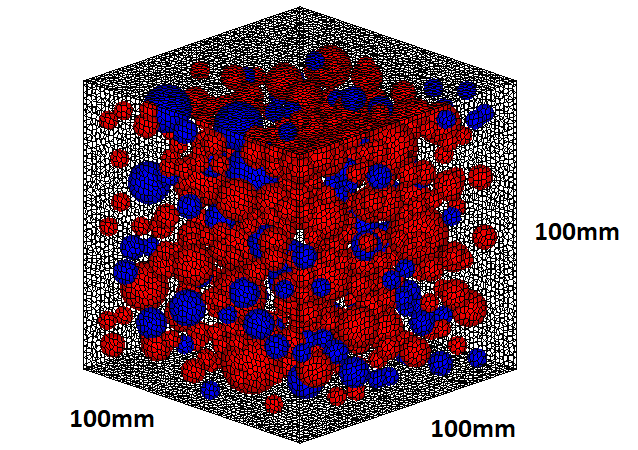
\includegraphics[width=.6\linewidth]{Files/Aggregate/A15P75.png}
  \caption{15\% Coarse Aggregate}
  \label{fig:A15_model}
\end{subfigure}%
\begin{subfigure}{.5\textwidth}
  \centering
  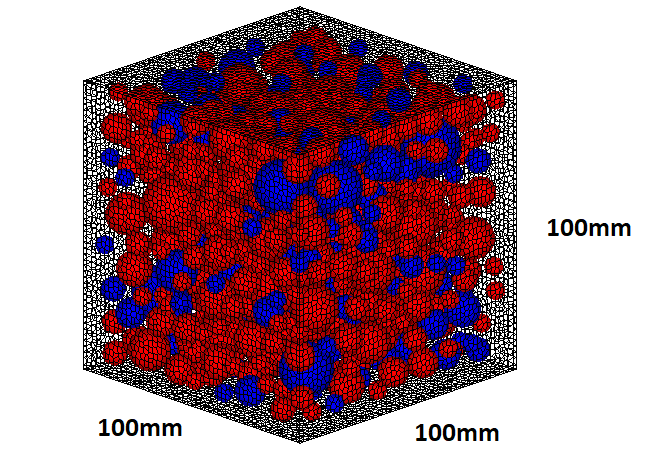
\includegraphics[width=.6\linewidth]{Files/Aggregate/A30P75.png}
  \caption{30\% Coarse Aggregate}
  \label{fig:A15_model}
\end{subfigure}
\caption{Coarse Aggregate Percentage}
\label{fig:Aggregate_Percentage}
\end{figure}

After modeling, similar ASR expansion simulations are carried out in the same way discribed in the previous section. Initial strain is giving to the interfaces between ASR reactive aggregate and paste, various from 0 to 0.003mm in each step to reach different level of global expansion in step 20.


From Table \ref{table:ASR_15vs30_EXP} can be seen that with same expansion step and same initial strain given in each step, the global expansion of with more coarse aggregate (A30 cases here) is higher than less coarse aggregate cases (A15 cases here).  As coarse aggregate ratio increased, ASR reactive interfaces are also increased, which suggested the reason for achieving larger global expansion in higher coarse aggregate cases.

This difference becomes more significant as the increasing of initial strain in each step, indicate that the amount of global expansion is not only depended on the amount of initial strain giving but also affected by other factors.


\begin{table}[ht!]
\centering
\begin{tabular}{ ||p{2cm}|p{2cm}|p{2cm}|p{2cm}|| }
 \hline
    Initial Strain (Each Step) & Expanding Steps & A15 Final Expansion & A30 Final Expansion[\%] \\ [0.5ex]
 \hline\hline
  0 & 0 & 0 & 0 \\
  0.0002 & 20 & 0.0699 & 0.0699\\
  0.0005 & 20 & 0.1364 & 0.1936\\
  0.001 & 20 & 0.3051 & 0.4223\\
  0.002 & 20 & 0.6290 & 0.8832\\
  0.003 & 20 & 0.9243 & 1.3224\\
 \hline
\end{tabular}
\caption{One Dimensional Expansion Ratio in Single ASR Model Simulation}
\label{table:ASR_15vs30_EXP}
\end{table}

%TODO:
Figure, plot of inital strain vs. global expansion ratio

\begin{figure}[!h]
\centering

    %*******
    \begin{subfigure}{.5\textwidth}
      \centering
      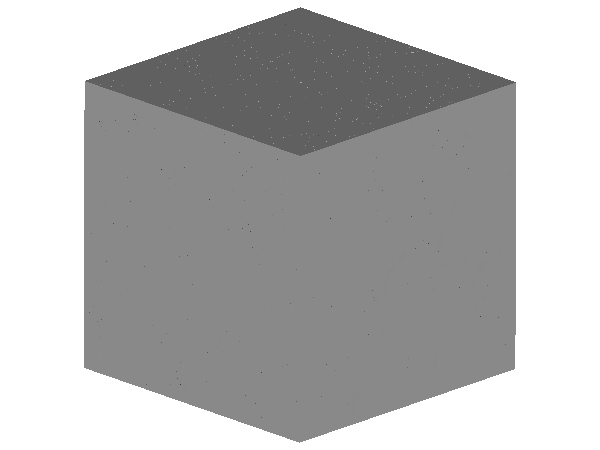
\includegraphics[width=.8\linewidth]{Files/exp_3D/ASR/A30Undamaged.png} %TODO: Fix. Should be A15
    \caption{Case 0: 0\% Expansion}
    \end{subfigure}%
    %*******
    \begin{subfigure}{.5\textwidth}
      \centering
      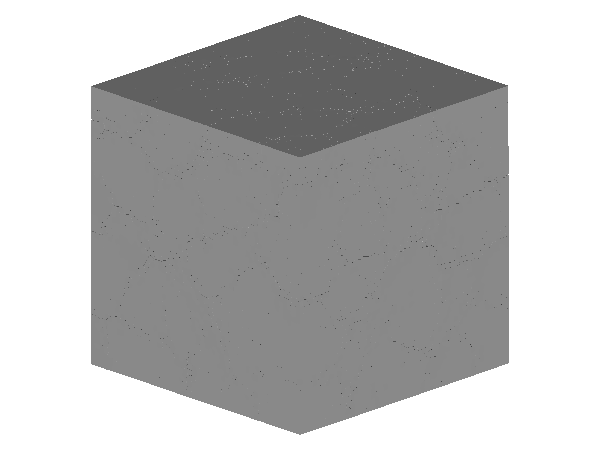
\includegraphics[width=.8\linewidth]{Files/exp_3D/ASR/A15P75_1_3d.png}
    \caption{Case 1: 0.0699\% Expansion}
    \end{subfigure}
    %*******
    \begin{subfigure}{.5\textwidth}
      \centering
      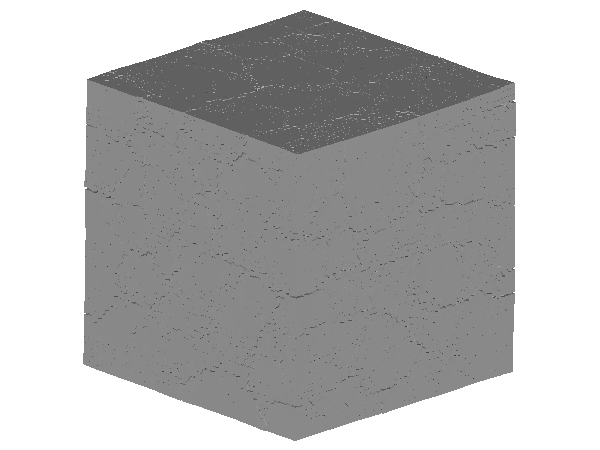
\includegraphics[width=.8\linewidth]{Files/exp_3D/ASR/A15P75_2_3d.png}
    \caption{Case 2: 0.1364\% Expansion}
    \end{subfigure}%
    %*******
    \begin{subfigure}{.5\textwidth}
      \centering
      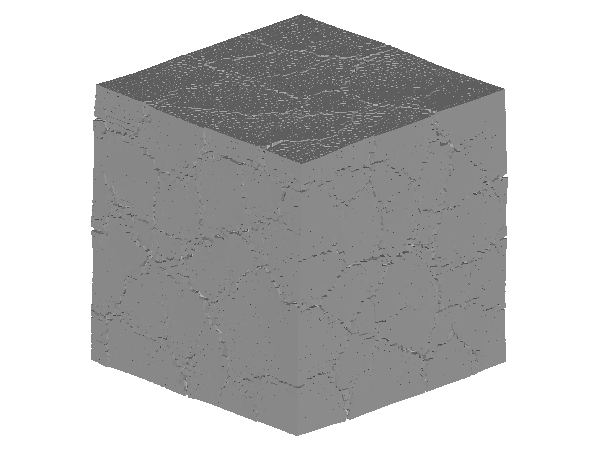
\includegraphics[width=.8\linewidth]{Files/exp_3D/ASR/A15P75_3_3d.png}
    \caption{Case 3: 0.3051\% Expansion}
    \end{subfigure}
    %*******
    \begin{subfigure}{.5\textwidth}
      \centering
      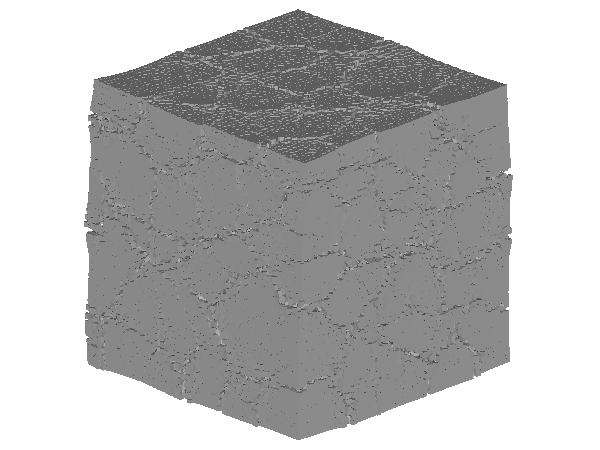
\includegraphics[width=.8\linewidth]{Files/exp_3D/ASR/A15P75_4_3d.png}
    \caption{Case 4: 0.629\% Expansion}
    \end{subfigure}%
    %*******
    \begin{subfigure}{.5\textwidth}
      \centering
      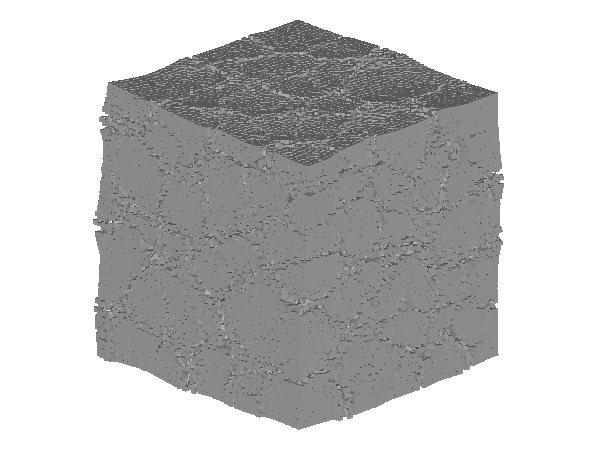
\includegraphics[width=.8\linewidth]{Files/exp_3D/ASR/A15P75_5_3d.png}
    \caption{Case 5: 0.9243\% Expansion}
    \end{subfigure}
    %*******

  \caption{3D Surface Cracks}
  \label{fig:ASR_A15P75_3D}
\end{figure}

% Surface of one side
\begin{figure}[!h]
\centering

    %*******
    \begin{subfigure}{.5\textwidth}
      \centering
      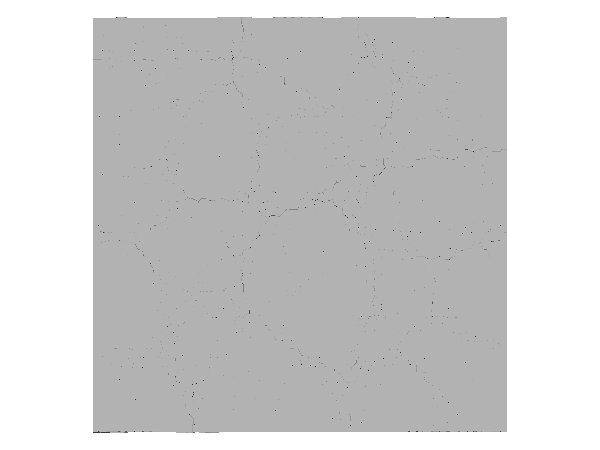
\includegraphics[width=.8\linewidth]{Files/exp_3D/ASR/A15P75_1_3ds.png}
    \caption{Case 0: 0\% Expansion}
    \end{subfigure}%
    %*******
    \begin{subfigure}{.5\textwidth}
      \centering
      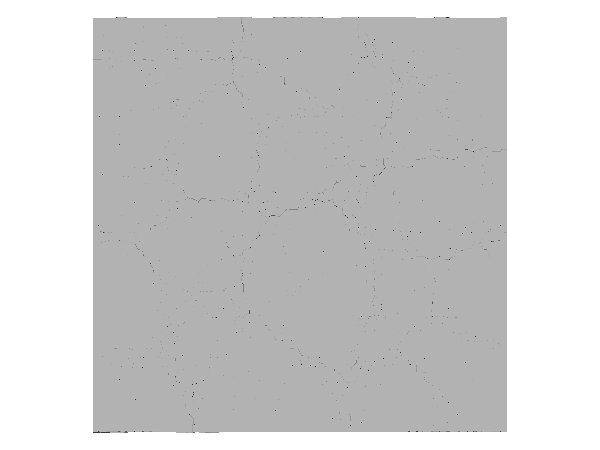
\includegraphics[width=.8\linewidth]{Files/exp_3D/ASR/A15P75_1_3ds.png}
    \caption{Case 1: 0.0699\% Expansion}
    \end{subfigure}
    %*******
    \begin{subfigure}{.5\textwidth}
      \centering
      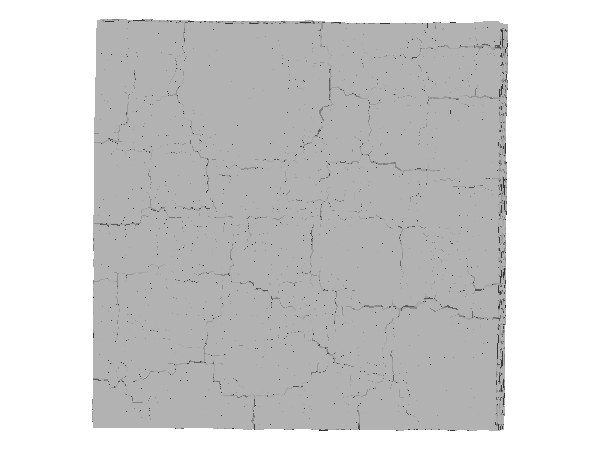
\includegraphics[width=.8\linewidth]{Files/exp_3D/ASR/A15P75_2_3ds.png}
    \caption{Case 2: 0.1364\% Expansion}
    \end{subfigure}%
    %*******
    \begin{subfigure}{.5\textwidth}
      \centering
      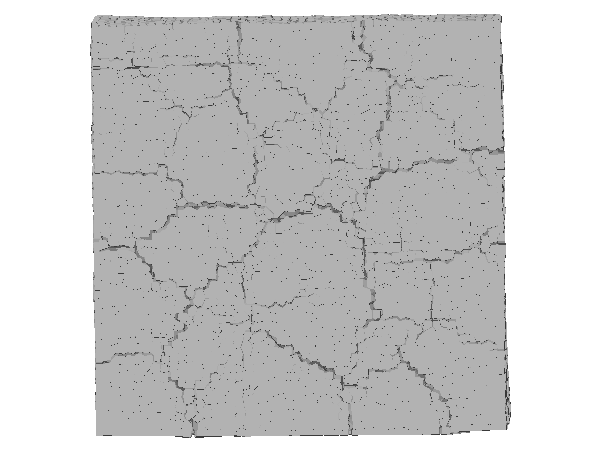
\includegraphics[width=.8\linewidth]{Files/exp_3D/ASR/A15P75_3_3ds.png}
    \caption{Case 3: 0.3051\% Expansion}
    \end{subfigure}
    %*******
    \begin{subfigure}{.5\textwidth}
      \centering
      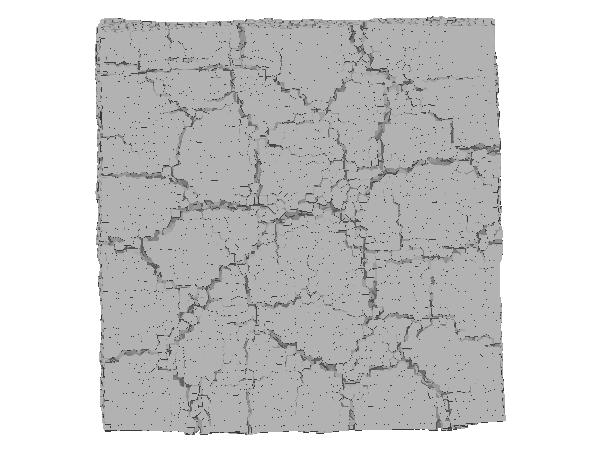
\includegraphics[width=.8\linewidth]{Files/exp_3D/ASR/A15P75_4_3ds.png}
    \caption{Case 4: 0.629\% Expansion}
    \end{subfigure}%
    %*******
    \begin{subfigure}{.5\textwidth}
      \centering
      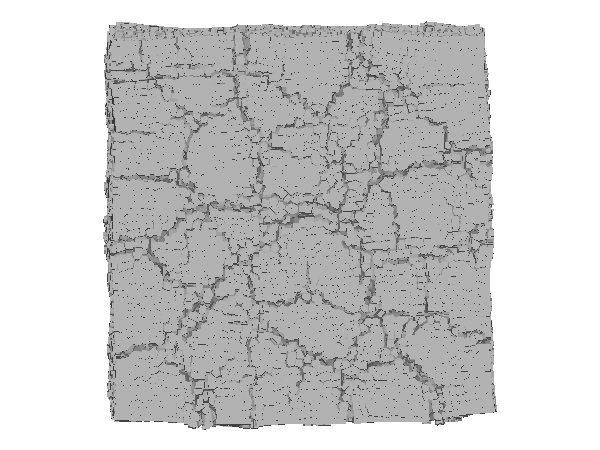
\includegraphics[width=.8\linewidth]{Files/exp_3D/ASR/A15P75_5_3ds.png}
    \caption{Case 5: 0.9243\% Expansion}
    \end{subfigure}
    %*******

  \caption{3D Surface Cracks (Single Side View)}
  \label{fig:ASR_A15P75_3DS}
\end{figure}

Figure \ref{fig:ASR_A15P75_3D} and Figure \ref{fig:ASR_A15P75_3DS} show surface crack pattern after ASR expansion of 15\% coarse aggregate cases.

Here 2 cases from 15\% coarse aggregate model and 30\% coarse aggregate model in relatively close global expansion rate are compared to show the influence of coarse aggregate ratio on cracking pattern.

For the aggregate ratio of 15\% model, case 3 is chosen, giving 0.001mm initial strain for ASR reactive interfaces, and reached 0.3051\% one-dimensional expansion after 20 steps. And for the aggregate ratio of 30\% model, case 3 is chosen, giving 0.001mm initial strain for ASR reactive interfaces and reached 0.4223\% one-dimensional expansion after 20 steps.


As can be seen in Figure \ref{fig:ASR_A15vsA30P75_3D}, at a relatively close global expansion ratio, the cracks are more concentrated with less coarse aggregate ratio case (aggregate 15\% here). This indicated that the concentration of location generate expansion could result in the concentration of global cracking distribution. Similar trend is also shown when decreasing the ratio of ASR reactive coarse aggregate ratio, which will be discussed later.

Both of the cases show clear characteristic map cracking which normally observed in ASR expanded concrete structures.

\begin{figure}[ht!]
\centering

    %*******
    \begin{subfigure}{.5\textwidth}
      \centering
      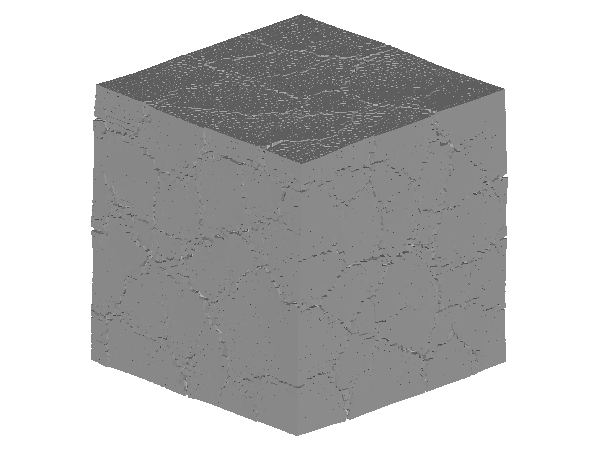
\includegraphics[width=.8\linewidth]{Files/exp_3D/ASR/A15P75_3_3d.png}
    \caption{A15 Case 3: 0.3051\% Expansion \\ 3D Surface Crack}
    \end{subfigure}%
    %*******
    \begin{subfigure}{.5\textwidth}
      \centering
      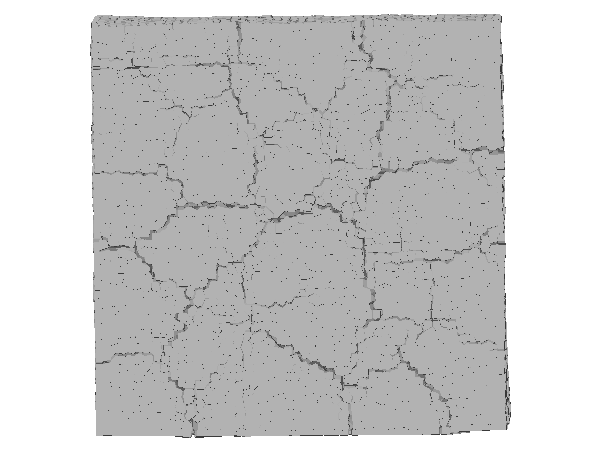
\includegraphics[width=.8\linewidth]{Files/exp_3D/ASR/A15P75_3_3ds.png}
    \caption{A15 Case 3: 0.3051\% Expansion \\ 3D Surface Cracks (Single Side View)}
    \end{subfigure}
    %*******
    \begin{subfigure}{.5\textwidth}
      \centering
      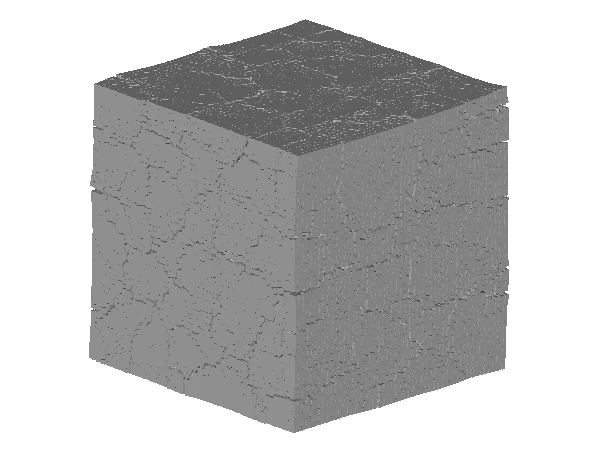
\includegraphics[width=.8\linewidth]{Files/exp_3D/ASR/A30P75_3_3d.png}
    \caption{A30 Case 3: 0.4223\% Expansion\\ 3D Surface Crack}
    \end{subfigure}%
    %*******
    \begin{subfigure}{.5\textwidth}
      \centering
      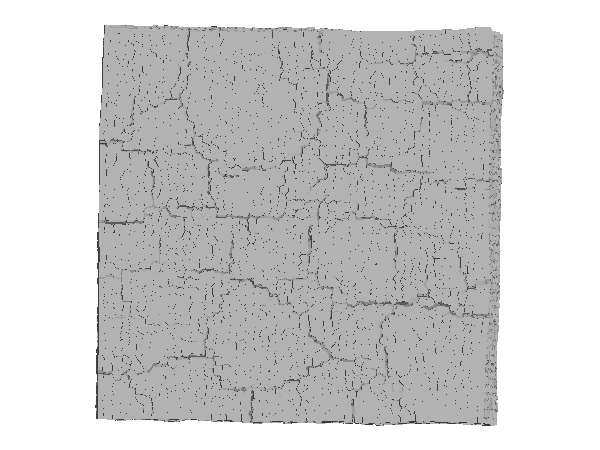
\includegraphics[width=.8\linewidth]{Files/exp_3D/ASR/A30P75_3_3ds.png}
    \caption{A30 Case 3: 0.4223\% Expansion\\ 3D Surface Cracks (Single Side View)}
    \end{subfigure}
    %*******

  \caption{Comparing Between A15 and A30 3D Surface Cracks}
  \label{fig:ASR_A15vsA30P75_3D}
\end{figure}

% Inner 3D Cracks
\begin{figure}[!h]
\centering

    %*******
    \begin{subfigure}{.5\textwidth}
      \centering
      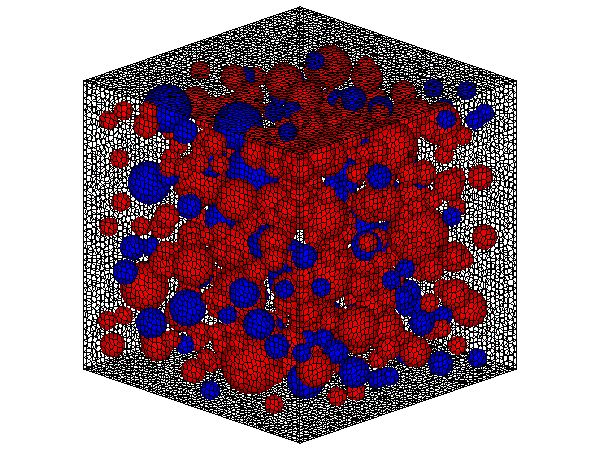
\includegraphics[width=.8\linewidth]{Files/exp_3D/ASR/A15P75_1_c.png}
    \caption{Case 0: 0\% Expansion}
    \end{subfigure}%
    %*******
    \begin{subfigure}{.5\textwidth}
      \centering
      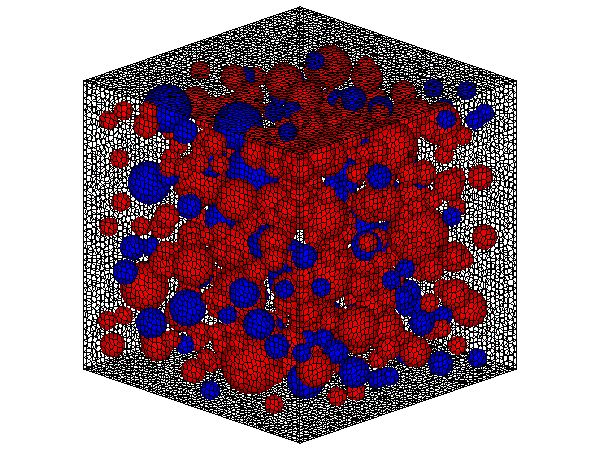
\includegraphics[width=.8\linewidth]{Files/exp_3D/ASR/A15P75_1_c.png}
    \caption{Case 1: 0.0699\% Expansion}
    \end{subfigure}
    %*******
    \begin{subfigure}{.5\textwidth}
      \centering
      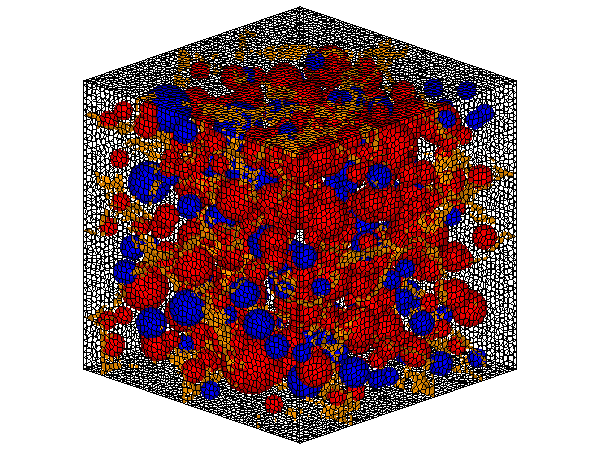
\includegraphics[width=.8\linewidth]{Files/exp_3D/ASR/A15P75_2_c.png}
    \caption{Case 2: 0.1364\% Expansion}
    \end{subfigure}%
    %*******
    \begin{subfigure}{.5\textwidth}
      \centering
      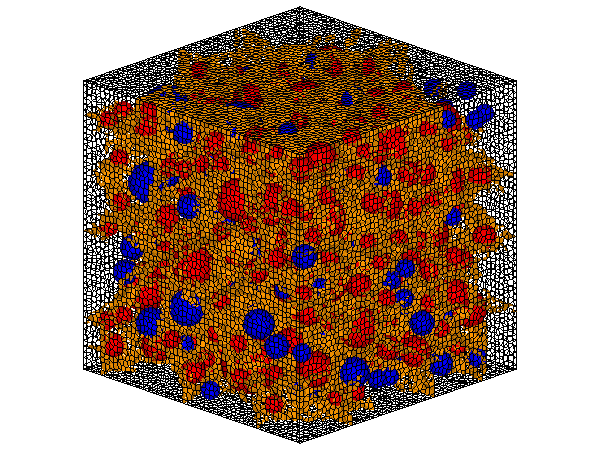
\includegraphics[width=.8\linewidth]{Files/exp_3D/ASR/A15P75_3_c.png}
    \caption{Case 3: 0.3051\% Expansion}
    \end{subfigure}
    %*******
    \begin{subfigure}{.5\textwidth}
      \centering
      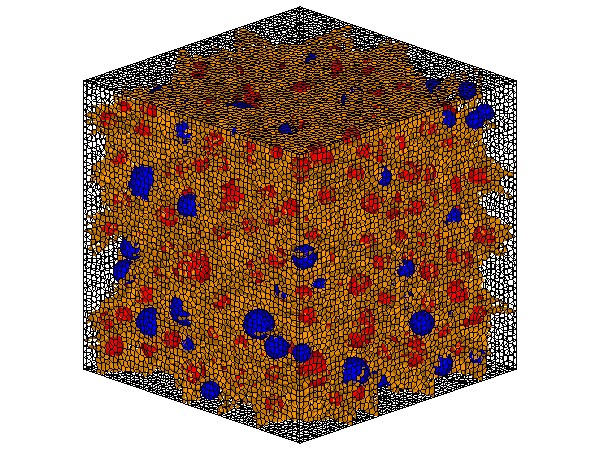
\includegraphics[width=.8\linewidth]{Files/exp_3D/ASR/A15P75_4_c.png}
    \caption{Case 4: 0.629\% Expansion}
    \end{subfigure}%
    %*******
    \begin{subfigure}{.5\textwidth}
      \centering
      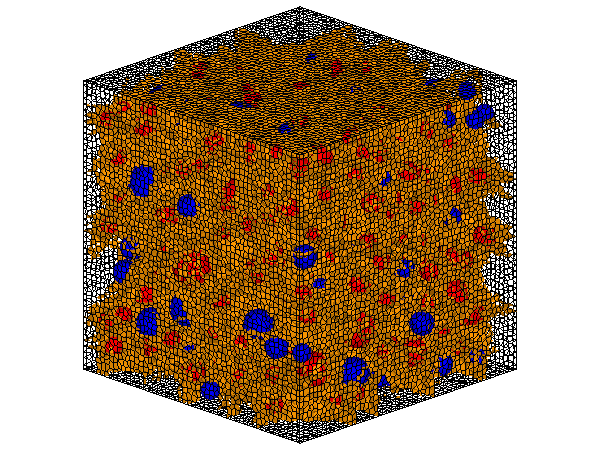
\includegraphics[width=.8\linewidth]{Files/exp_3D/ASR/A15P75_5_c.png}
    \caption{Case 5: 0.9243\% Expansion}
    \end{subfigure}
    %*******

  \caption{3D Inner Crack Width Larger than 0.03mm}
  \label{fig:ASR_A15P75_crack}
\end{figure}

In Figure \ref{fig:ASR_A15P75_crack}, here if compare the inner crack of two cases at a relatively close global expansion ratio, the cracks larger than 0.03mm are generally more with less coarse aggregate ratio case (aggregate 15\% here). 



\begin{table}[!h]
\centering
\begin{tabular}{ ||p{4cm}|p{4cm}|p{4cm}|| }
\hline
 Crack Width [mm] &  A15 Case 3 Total Cracked Interfaces &  A30 Case 3 Total Cracked Interfaces \\
 \hline\hline

   0.00000 - 0.00005 & 363340 & 316744 \\
   0.00005 - 0.00010 & 303804 & 286704 \\
   0.00010 - 0.00020 & 263111 & 263943 \\
   0.00020 - 0.00050 & 220320 & 234672 \\
   0.00050 - 0.00100 & 163316 & 183238 \\
   0.00100 - 0.00300 & 117764 & 131553 \\
   0.00300 - 0.01000 & 45969 & 42432 \\
   0.01000 - 0.03000 & 696 & 275 \\
   0.03000 - 0.10000 & 0 & 0 \\
   0.1000+ & 0 & 0 \\

  \hline
  \end{tabular}
\caption{Expansion in Each Step for A15P75 Case 3 and A30 P75 Case 3}
\label{table:A15vsA30P75_3_Cracks}
\end{table}

% TODO: stack bar plot for A15vsA30P75_3_Cracks

If comparing the distribution of cracks summarised by its crack width (Table \ref{table:A15vsA30P75_3_Cracks}),  it can be seen that the distribution pattern is relatively close for 15\% coarse aggregate case with 0.3051\% global expansion and  30\% coarse aggregate case with 0.4223\% global expansion.  The number of cracked faces decrease gradually when increasing the crack width.

However, if compare closer on relatively larger cracks, cracking face number of the case with 15\% coarse aggregate is higher. For example, for the number of cracked interfaces larger than 0.003mm, 15\% coarse aggregate case is 9.27\% higher than 30\% coarse aggregate case. And for the number of cracked interfaces larger than 0.01mm, 15\% coarse aggregate case is 2.53 times of 30\% coarse aggregate case.  Those larger cracks having more significant influence when the global cracking patterns are compared and should distribute more when considering the damage on the concrete structure.
\begin{figure}[h!]
\centering

    %*******
    \begin{subfigure}{.5\textwidth}
      \centering
      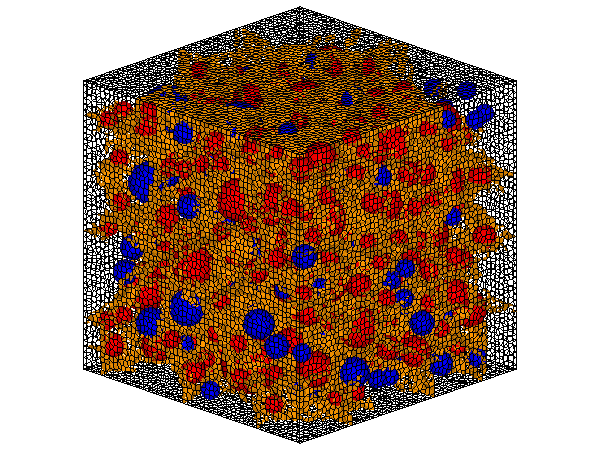
\includegraphics[width=.8\linewidth]{Files/exp_3D/ASR/A15P75_3_c.png}
    \caption{A15 Case 3: 0.3051\% Expansion \\ 3D Inner Crack}
    \end{subfigure}%
    %*******
    \begin{subfigure}{.5\textwidth}
      \centering
      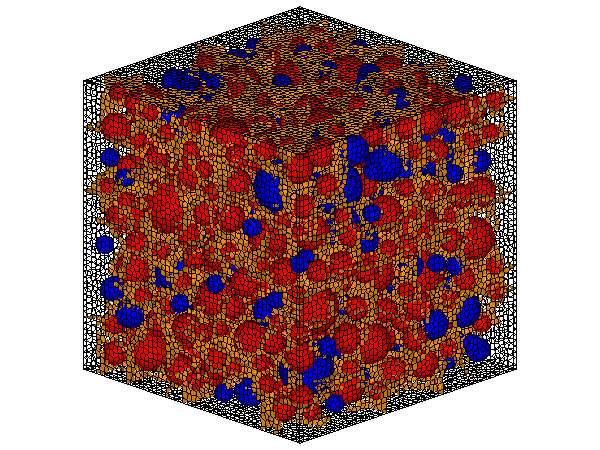
\includegraphics[width=.8\linewidth]{Files/exp_3D/ASR/A30P75_3_c.png}
    \caption{A30 Case 3: 0.4223\% Expansion \\ 3D Inner Cracks}
    \end{subfigure}

  \caption{Comparing Between A15 and A30 3D Surface Cracks}
  \label{fig:ASR_A15vsA30P75_3D}
\end{figure}
